\documentclass[tikz,border=5mm]{standalone}
\usepackage{tikz}
\usetikzlibrary{calc}

\begin{document}
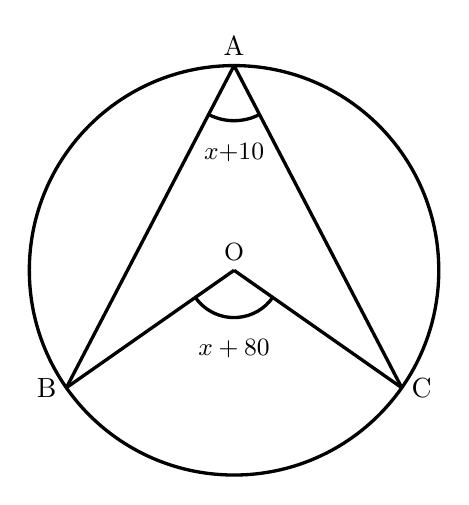
\begin{tikzpicture}[scale=2]

% Define the radius
\def\r{1.3}

% Center of circle
\coordinate (O) at (0,0);

% Draw the circle
\draw[very thick] (O) circle (\r);

% Define vertices on the circle
% Using specific angles for symmetry
\coordinate (A) at (90:\r);
\coordinate (B) at (215:\r);
\coordinate (C) at (325:\r);

% Draw triangle sides
\draw[very thick] (A) -- (B);
\draw[very thick] (A) -- (C);

% Draw radii from center O to B and C
\draw[very thick] (O) -- (B);
\draw[very thick] (O) -- (C);

% Calculate angles at A
% Angle from A to B
\pgfmathsetmacro{\angleAtoB}{atan2(sin(215)*\r - sin(90)*\r, cos(215)*\r - cos(90)*\r)}
% Angle from A to C
\pgfmathsetmacro{\angleAtoC}{atan2(sin(325)*\r - sin(90)*\r, cos(325)*\r - cos(90)*\r)}

% Angle arc at A (x+10) - perfectly fitted
\def\arcRadA{0.35}
\draw[very thick] ($(A)+({\angleAtoB}:\arcRadA)$) arc[start angle=\angleAtoB, end angle=\angleAtoC, radius=\arcRadA];
\node at ($(A)+(0,-0.55)$) {\small $x{+}10$};

% Angle arc at O (x+80) - perfectly fitted
\def\arcRadO{0.3}
\draw[very thick] ($(O)+(215:\arcRadO)$) arc[start angle=215, end angle=325, radius=\arcRadO];
\node at ($(O)+(0,-0.5)$) {\small $x + 80$};

% Vertex labels
\node[above] at (A) {A};
\node[left] at (B) {B};
\node[right] at (C) {C};
\node[above] at (O) {\small O};

\end{tikzpicture}
\end{document}